\documentclass[12pt, a4paper]{extarticle}
\usepackage{geometry}
\geometry{
	a4paper,
	total={170mm,257mm},
	left=20mm,
	top=20mm,
	}
\usepackage{graphicx, float} % For figures
\usepackage{authblk}

%title and author details
\title{Aeroelastic Analysis of Hypersonic Double-wedge Lifting Surface}
\author[1]{Koorosh Gobal}
\author[1]{Anusha Anisetti}
\author[1]{Vana Naga Samyuktha Nuthy}
\affil[1]{Department of Mechanical and Materials Engineering, Wright State University}
\date{} %remove date

\begin{document}

\maketitle

\abstract{This work presents a treatment of the hypersonic aeroelastic problem using Piston theory as aerodynamic model. The wing is modeled as a double-wedge with pitching degree of freedom. The steady-state response of such nonlinear systems is typically solved by time-integration of finite element models. The drawback of such time-domain methods is the excessive need for computational time and resources. This can become a major bottle neck in design space exploration efforts of such systems where mutiple solutions for different configurations is needed. In this work we use harmonic balance method, which transforms and solves the underlying equation of motion in the frequency domain. This can reduce the simulation cost by orders of magnitude. This methodology is first build on a closed form equation for structural response and later extended to a generic hypersonic vehicle model of \cite{oppenheimer2007flexible} where the structural response is calculated using finite element method.}
% ===================================================================
\section{Introduction}
With renewed interest in space operations worldwide, there is an interest in hypersonic coupled aero-structural research. The combined effects of a flexible vehicle travelling at high speeds and subjected to large forces may lead to significant unsteady aerodynamic effects. Hence, understanding the concepts and consequences of time-dependent response of the system is critical to the successful development of this type of vehicle.

Nonlinear coupled aero-structural analysis plays an important role in the aerospace industry however, there are no efficient methods available for a nonlinear structural frequency response analysis. Most of the aviable methods are based on time domain analysis which require excessive amount of computational resources. This has become a major bottleneck in design space exploration and optimization of such systems.

The harmonic balance method (HBM), transforms and solves the underlying equation of motion in the frequency domain. If done right, major reduction in computational time can be achieved using this approach. Though harmonic balance is a well-established method for nonlinear frequency analysis, for example in the context of integrated circuit simulations \cite{gilmore1991nonlinear}, it is so far hardly used in mechanics, only for lower dimensional structural models such as beams and plates \cite{ribeiro2004non}. Commerical finite element analysis (FEA) software such as ANSYS, Nastran or ABAQUS do not provide any methods dedicated to nonlinear frequency response. %This is mainly due to the truncated Fourier expansion HBM uses for frequency domain approximation of each degree of freedom (DOF) of the spatial discretization, which produces a blow-up of total DOFs: the sparse linear system to be solved in the end is not only m-times bigger, but also with m-times as many non-zero entries per row as the spatial discretization, where m is the number of Fourier coefficients. Therefore we need model order reduction (MOR) of the spatial discretization to reduce the size of the linear system significantly and make an efficient numerical solution of the system arising from HBM even possible.

In this work, piston theory is applied to a double-wedged lifting surface with pitching degree of freedom as shown in Figure \ref{fig:doubleWedgedAirfoil}. This work uses third-order piston theory to compute unsteady effects behind shock waves and expansion fans and a stiffening spring to the structure. This method of computing unsteady aerodynamic effects delivered highly accurate results when compared to computational fluid dynamics solutions \cite{mcnamara2011aeroelastic}.

\begin{figure}[h]
	\centering
	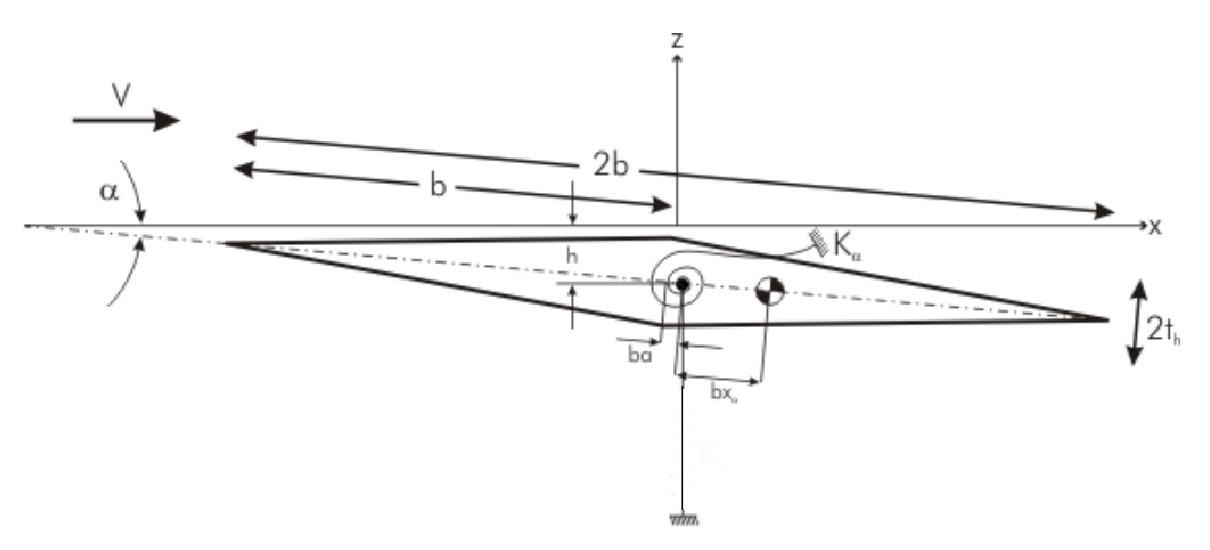
\includegraphics[width=7.00cm]{figure/doubleWedgeAirfoil.png}
	\caption{Double-wedge lifting surface.}
	\label{fig:doubleWedgedAirfoil}
\end{figure}
% ===================================================================
\section{Piston Theory}

% ===================================================================
\bibliographystyle{unsrt}
\bibliography{ref}
\end{document}